\documentclass[12pt]{article}
\usepackage{url, graphicx, epstopdf, amsmath, esint}
\usepackage{physics}

% page layout
\setlength{\topmargin}{-0.25in}
\setlength{\textheight}{9.5in}
\setlength{\headheight}{0in}
\setlength{\headsep}{0in}
\setlength{\parindent}{1.1\baselineskip}
\addtolength{\oddsidemargin}{-0.75in}
\setlength{\marginparwidth}{2in}

% problem formatting
\newcommand{\problemname}{Problem}
\newcounter{problem}
\newcommand{\startproblem}{\paragraph{Problem~\theproblem:}\refstepcounter{problem}}

% words
\newcommand{\foreign}[1]{\textsl{#1}}
\newcommand{\vs}{\foreign{vs}}

% math
\renewcommand{\vec}[1]{\boldsymbol{#1}}
% \newcommand{\dd}{\mathrm{d}} % PROVIDED IN physics PACKAGE
\newcommand{\e}{\mathrm{e}}
% \newcommand{\cross}{\times} % PROVIDED IN physics PACKAGE
% \newcommand{\curl}{\vec{\nabla}\times} % PROVIDED IN physics PACKAGE

% primary units
\newcommand{\rad}{\mathrm{rad}}
\newcommand{\kg}{\mathrm{kg}}
\newcommand{\m}{\mathrm{m}}
\newcommand{\s}{\mathrm{s}}
\newcommand{\A}{\mathrm{A}}

% secondary units
\renewcommand{\deg}{\mathrm{deg}}
\newcommand{\km}{\mathrm{km}}
\newcommand{\cm}{\mathrm{cm}}
\newcommand{\mm}{\mathrm{mm}}
\newcommand{\mum}{\mathrm{\mu m}}
\newcommand{\nm}{\mathrm{nm}}
\newcommand{\ft}{\mathrm{ft}}
\newcommand{\mi}{\mathrm{mi}}
\newcommand{\AU}{\mathrm{AU}}
\newcommand{\ns}{\mathrm{ns}}
\newcommand{\h}{\mathrm{h}}
\newcommand{\yr}{\mathrm{yr}}
\newcommand{\N}{\mathrm{N}}
\newcommand{\J}{\mathrm{J}}
\newcommand{\eV}{\mathrm{eV}}
\newcommand{\MeV}{\mathrm{MeV}}
\newcommand{\W}{\mathrm{W}}
\newcommand{\Pa}{\mathrm{Pa}}
\newcommand{\C}{\mathrm{C}}
\newcommand{\V}{\mathrm{V}}
\newcommand{\ohm}{\mathrm{\Omega}}
\newcommand{\muF}{\mathrm{\mu F}}
\newcommand{\Hz}{\mathrm{Hz}}
\newcommand{\GHz}{\mathrm{GHz}}

% derived units
\newcommand{\mps}{\m\,\s^{-1}}
\newcommand{\mph}{\mi\,\h^{-1}}
\newcommand{\mpss}{\m\,\s^{-2}}
\newcommand{\radps}{\rad\,\s^{-1}}

% random stuff
\sloppy\sloppypar\raggedbottom\frenchspacing\thispagestyle{empty}

\begin{document}

\section*{NYU Physics 2---Problem Set 5}

Due Thursday 2022 March 03 by 12:30\,pm on Brightspace.

\paragraph{Problem~\theproblem:}\refstepcounter{problem}%
Look up the dielectric constants for materials.
In standard, inexpensive, commercial capacitors, what kinds of dielectrics are used?
How much lower would the capacitances be for those capacitors if the gaps were air gaps instead
of dielectric-filled gaps?
Are there materials with dielectric constants in the thousands? If so, what are their properties?

\paragraph{Problem~\theproblem:}\refstepcounter{problem}%
In this circuit, resistor $R_3$ is variable; that is, you can tune it. At what value of $R_3$
is the current through resistor $R$ exactly zero? What happens if $R_3$ is
greater than this resistance? Which way does the current flow through resistor $R$ and what is
the magnitude of the current?
\marginpar{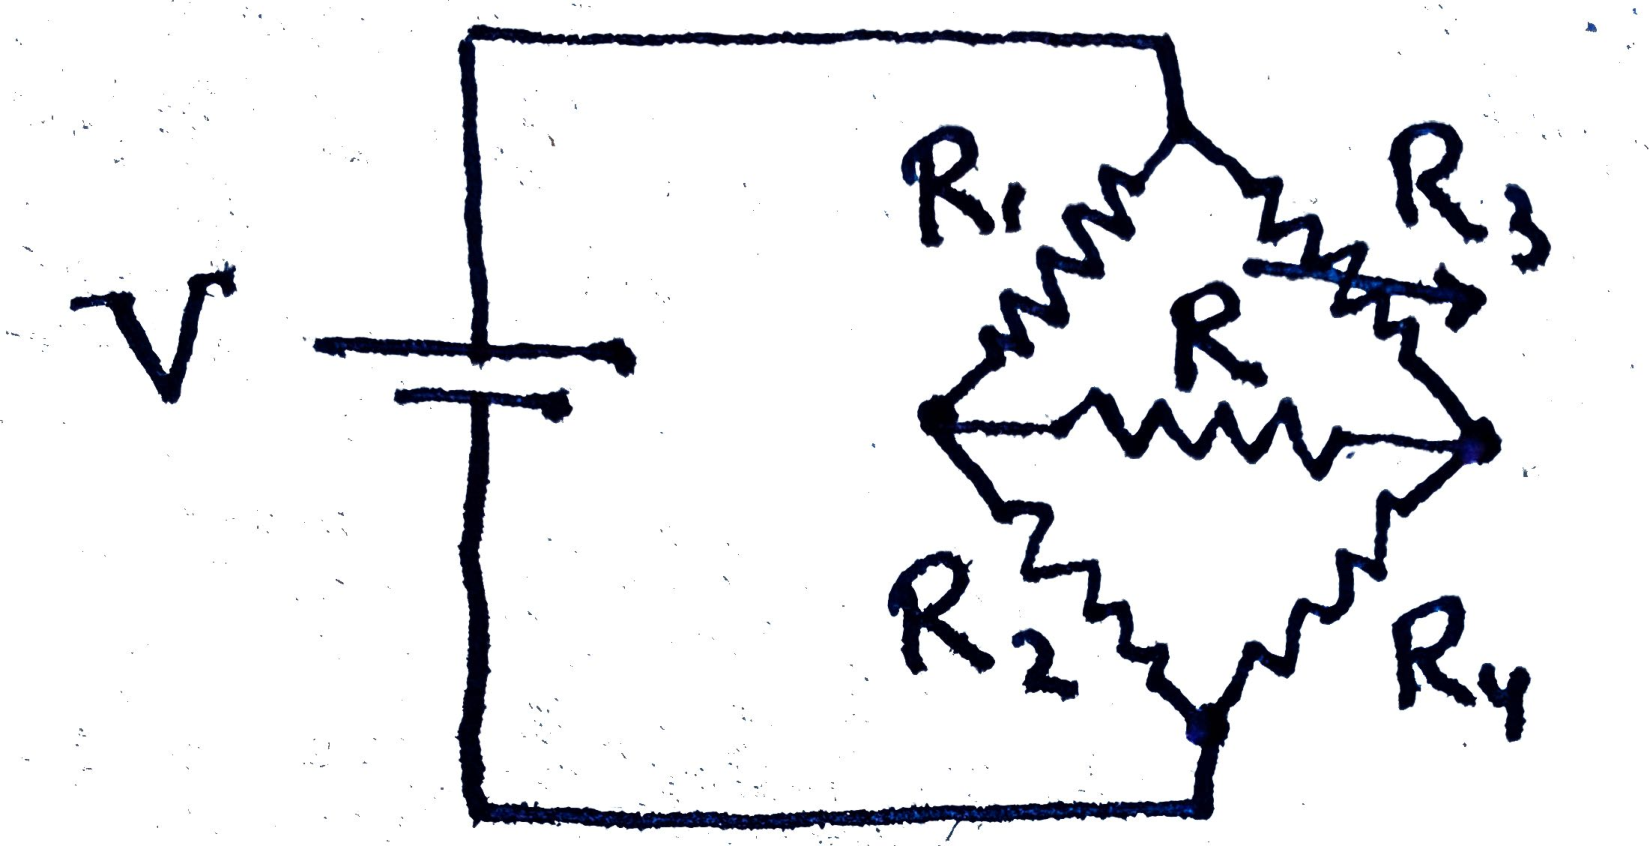
\includegraphics[width=\marginparwidth]{bridge.pdf}}

\paragraph{Problem~\theproblem:}\refstepcounter{problem}%
A circuit consists of a capacitor $C$ and a resistor $R$,
and nothing else.
At time $t=0$, the capacitor contains charge $q_0$.
What is the instantaneous flow of current $I_0$ in the circuit at time $t=0$?
As time goes on, charge will flow and the capacitor will discharge.
Write down the equation relating $q(t)$ and its time derivative $\dd q/\dd t$ (which
is related to the current) and show that this equation is satisfied if the charge
as a function of time is given by
\begin{equation}
q(t) = q_0\,\exp \alpha\,t
\end{equation}
where $\alpha$ has some expression in terms of $R$ and $C$. What is that expression?

\paragraph{Problem~\theproblem:}\refstepcounter{problem}%
Consider a parallel-plate capacitor of $x$-direction width $X$,
$y$-direction depth $Y$ and $z$-direction plate
separation $h$, charged to a total charge $\pm Q$, filled with a slab of
dielectric of constant $\kappa$.  If you pull
the dielectric slab out of the capacitor by a distance $x$, you change
the capacitance. Compute the capacitance $C$ and
total energy $U$ in the capacitor as a function of $x$. You will have to
ignore edge effects---that is, assume that the separation is very small
relative to all other dimensions.

\textsl{Bonus part, not for credit:} Compute the
force $F$ required as a function of $x$ to remove the slab.
Remember: Forces are spatial derivatives of energies!

\textsl{Bonus part, not for credit:} How do your answers change if you
hold the voltage $V$ on the capacitor fixed instead of the charge $Q$?

\end{document}
